\documentclass[12pt]{article}
\usepackage{lingmacros}
\usepackage{tree-dvips}
\usepackage{graphicx} %package to manage images
\usepackage{float}
\usepackage{subcaption}%package for enabling multiple images in a single figure
\graphicspath{ {/} }
\begin{document}

\section*{Question 1}

\begin{figure}[H]
    \centering
    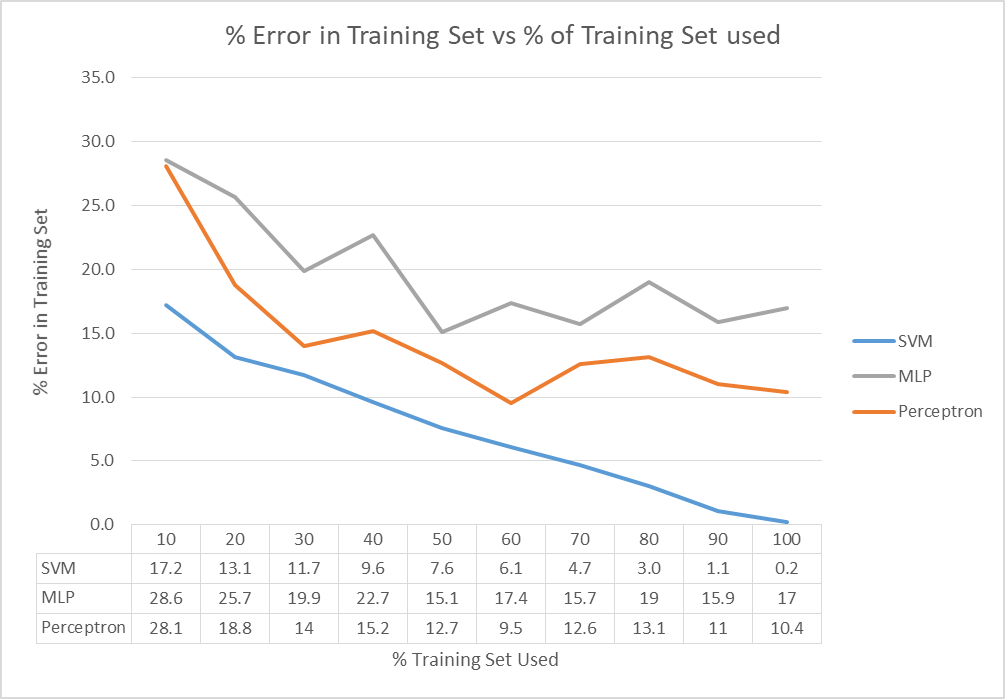
\includegraphics[width=1\textwidth]{question_1_3}
    \caption{A graph showing percent correct of the training set as a function of the percentage of the training set used.}
    \label{fig:question_1_3}
\end{figure}

\begin{figure}[H]
    \centering
    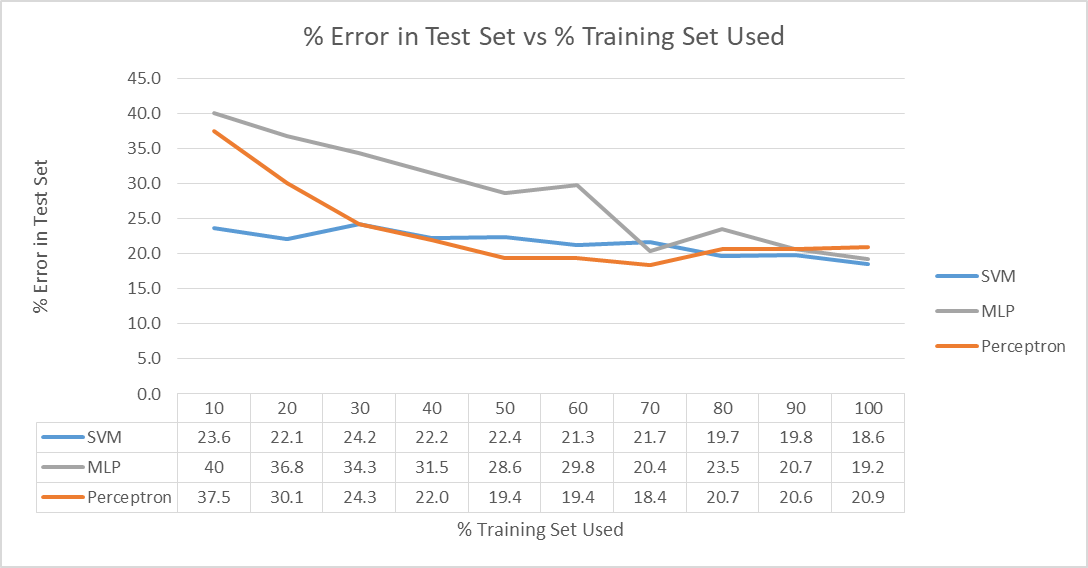
\includegraphics[width=1\textwidth]{question_1_4}
    \caption{A graph showing percent correct of the test set as a function of the percentage of the training set used.}
    \label{fig:question_1_4}
\end{figure}

Of the three algorithms tested, SVM appears to perform the best on both the training and test set, while MLP performs the worst. For perceptron, we took the dot product of the weights times the training data and selected the layer that had the highest dot product as our hypothesis. If the hypothesis was incorrect, then the training data was subtracted from the weights of the incorrect label and added to the weights of the correct label. For MLP, we used a softmax algorithm. The first layer takes the dot product of the weights times the training data and passes it as input to the softmax layer, which uses the following equation:

\begin{equation}
softmax(label = x) = \frac{e^{w_xt}}{\sum_{n=0}^{9}e^{w_nt}}
\end{equation}

Where t is the training data and there are 10 labels, 0-9. Then, the highest value of the softmax layer was used as the guess. If the hypothesis was incorrect, then the error was backpropagated to the weights layer by multiplying $y - h_w$ by $s(1-s)$, where y is the correct label, $h_w$ is the hypothesis, and s is the softmax value for that label. This was added to the weights for the correct and incorrect labels. SVM used the inbuilt SVM functions to maximize the margins between labels and guess that way. Overall, it seems like SVM overfit to the training data but still performed better than perceptron and MLP. MLP was the least well fit to the training data but still performed reasonably well on test data, indicating that it was more generalized than SVM. If SVM was trained on more data, there is a chance that it would have overfit to the data and actually performed worse than perceptron and MLP. MLP and perceptron on the other hand seem to have stagnated when 100\% data is used, showing very similar error rates from 50 - 100\% of the training data used. This may indicate that further training data may not greatly improve performance for MLP or perceptron.

\section*{Question 2}

\subsection*{Part a}

1) 4.0 GPA - P, the data match the decision tree\\
2) 3.9 GPA - P, the data match the decision tree\\
3) 3.9 GPA - P, the data match the decision tree\\
4) 3.8 GPA - yes publications - P, the data match the decision tree\\
5) 3.6 GPA - no publications - rank 2 university - P, the data match the decision tree\\
6) 3.6 GPA - yes publications - P, the data match the decision tree\\
7) 3.4 GPA - no publications - rank 3 university - N, the data match the decision tree\\
8) GPA 3.4 - No publication - Rank 1 University - N, data match the tree\\
9) GPA 3.2 - N, data match the tree\\
10) GPA 3.1 - N, data match the tree\\
11) GPA 3.1 - N, data match the tree\\
12) GPA 3.0 - N, data match the tree\\

\subsection*{Part b}
For the entire set, there are 6 positives and 6 negatives. Hence, the entropy of the set is:
\\
\begin{equation}
E(S) = -\frac{1}{2}\log_2\frac{1}{2} -\frac{1}{2}\log_2\frac{1}{2} = 1
\end{equation}
\\
For GPA, the information gained is:
\\
GPA >= 3.9: 3 P, 0 N
\begin{equation}
E(GPA >= 3.9) = -1\log_21 -0\log_20 = 0
\end{equation}
\\
3.2 < GPA < 3.9: 3 P, 2 N
\begin{equation}
E(3.2 < GPA < 3.9) = -\frac{3}{5}\log_2\frac{3}{5} -\frac{2}{5}\log_2\frac{2}{5} = 0.9710
\end{equation}
\\
GPA <= 3.2: 0 P, 4 N
\begin{equation}
E(GPA <= 3.2) = -0\log_20 -1\log_21 = 0
\end{equation}
\begin{equation}
I(GPA) = \frac{1}{4} * 0 + \frac{5}{12} * 0.9710 + \frac{1}{3} * 0 = 0.4046
\end{equation}
\begin{equation}
Gain(GPA) = E(S) - I(GPA) = 1 - 0.4046 = 0.5954
\end{equation}
\\
For university rank, the information gained is:
\\
University rank = 1: 3 P, 2 N
\begin{equation}
E(rank = 1) = -\frac{3}{5}\log_2\frac{3}{5} -\frac{2}{5}\log_2\frac{2}{5} = 0.9710
\end{equation}
\\
University rank = 2: 2 P, 1 N
\begin{equation}
E(rank = 2) = -\frac{2}{3}\log_2\frac{2}{3} -\frac{1}{3}\log_2\frac{1}{3} = 0.9183
\end{equation}
\\
University rank = 3: 1 P, 3 N
\begin{equation}
E(rank = 3) = -\frac{1}{4}\log_2\frac{1}{4} -\frac{3}{4}\log_2\frac{3}{4} = 0.8113
\end{equation}
\begin{equation}
I(rank) = \frac{5}{12} * 0.9710 + \frac{1}{4} * 0.9183 + \frac{1}{3} * 0.8113 = 0.9046
\end{equation}
\begin{equation}
Gain(rank) = E(S) - I(rank) = 1 - 0.9046 = 0.0954
\end{equation}
\\
For whether the student has publications, the information gained is:
\\
Published = Yes : 3 P, 2 N
\begin{equation}
E(Published = Yes) = -\frac{3}{5}\log_2\frac{3}{5}) - \frac{2}{5}\log_2\frac{2}{5} = .9710
\end{equation}
\\
Published = No : 3 P, 4 N
\begin{equation}
E(Published = No) = -\frac{3}{7}\log_2\frac{3}{7} - \frac{4}{7}\log_2\frac{4}{7} = .9852
\end{equation}
\begin{equation}
I(Published) = \frac{5}{12}(.9710)+\frac{7}{12}(.9852) = 0.9792
\end{equation}
\begin{equation}
Gain(Published) = E(S) - I(Published) = 1 - 0.9792 = 0.0208
\end{equation}
\\
For the quality of the student's recommendations, the information gained is:
\\
Recommendations = Good : 5 P, 3 N
\begin{equation}
E(Recommendations = Good) = -\frac{5}{8}\log_2\frac{5}{8}-\frac{3}{8}\log_2\frac{3}{8} = .9544
\end{equation}
\\
Recommendations = Normal : 1 P, 3 N
\begin{equation}
E(Recommendations = Normal) = -\frac{1}{4}\log_2\frac{1}{4}-\frac{3}{4}\log_2\frac{3}{4} = .8113
\end{equation}
\begin{equation}
I(Recommendations) = \frac{8}{12}(.9544)+\frac{4}{12}(.8113) = 0.9067
\end{equation}
\begin{equation}
Gain(Recommendations) = E(S) - I(Recommendations) = 1 - 0.9067 = 0.0933
\end{equation}
\\
For the root of the decision tree, the best attribute to use is GPA, since it has the highest information gain of all the attributes. Because a GPA of 4.0 always leads to P and a GPA of 3.3 always leads to N, we only need to investigate the next node for when GPA = 3.6.
\\
For the subset, there are 3 positives and 2 negatives. Hence, the entropy of the subset is:
\\
\begin{equation}
E(S) = -\frac{3}{5}\log_2\frac{3}{5} -\frac{2}{5}\log_2\frac{2}{5} = 0.9710
\end{equation}
\\
For university rank, the information gained is:
\\
University rank = 1 : 1 P, 1 N
\begin{equation}
E(rank = 1) = -\frac{1}{2}\log_2\frac{1}{2} -\frac{1}{2}\log_2\frac{1}{2} = 1
\end{equation}
\\
University rank = 2 : 1 P, 0 N
\begin{equation}
E(rank = 2) = -1\log_21 -0\log_20 = 0
\end{equation}
\\
University rank = 3 : 1 P, 1 N
\begin{equation}
E(rank = 3) = -\frac{1}{2}\log_2\frac{1}{2} -\frac{1}{2}\log_2\frac{1}{2} = 1
\end{equation}
\begin{equation}
I(rank) = \frac{2}{5} * 1 + \frac{1}{5} * 0 + \frac{2}{5} * 1 = 0.8
\end{equation}
\begin{equation}
Gain(rank) = E(S) - I(rank) = 0.9710 - 0.8 = 0.1710
\end{equation}
\\
For whether the student has publications, the information gained is:
\\
Published = Yes : 2 P, 0 N
\begin{equation}
E(Published = Yes) = -1\log_21 - 0\log_20 = 0
\end{equation}
\\
Published = No : 2 P, 1 N
\begin{equation}
E(Published = No) = -\frac{2}{3}\log_2\frac{2}{3} - \frac{1}{3}\log_2\frac{1}{3} = 0.9183
\end{equation}
\begin{equation}
I(Published) = \frac{2}{5}(0)+\frac{3}{5}(.9183) = 0.5510
\end{equation}
\begin{equation}
Gain(Published) = E(S) - I(Published) = 0.9710 - 0.5510 = 0.42
\end{equation}
\\
For the quality of the student's recommendations, the information gained is:
\\
Recommendations = Good : 3 P, 2 N
\begin{equation}
E(Recommendations = Good) = -\frac{3}{5}\log_2\frac{3}{5}) - \frac{2}{5}\log_2\frac{2}{5} = .9710
\end{equation}
\\
Recommendations = Normal : 0 P, 0 N
\begin{equation}
E(Recommendations = Normal) = -0\log_20-0\log_20 = 0
\end{equation}
\begin{equation}
I(Recommendations) = 1(.9710)+0(0) = 0.9710
\end{equation}
\begin{equation}
Gain(Recommendations) = E(S) - I(Recommendations) = 0.9710 - 0.9710 = 0
\end{equation}
\\
The best attribute to use next would be whether the student has publications. Because if the student has publications the answer is always positive, then we only need to examine when the student doesn't have publications to create the next child node in the decision tree.
\\
For the subset, there is 1 positive and 2 negatives. Hence, the entropy of the subset is:
\\
\begin{equation}
E(S) = -\frac{1}{3}\log_2\frac{1}{3} - \frac{2}{3}\log_2\frac{2}{3} = 0.9183
\end{equation}
\\
For university rank, the information gained is:
\\
University rank = 1 : 0 P, 1 N
\begin{equation}
E(rank = 1) = -0\log_20 - 1\log_21 = 0
\end{equation}
\\
University rank = 2 : 1 P, 0 N
\begin{equation}
E(rank = 2) = -1\log_21 -0\log_20 = 0
\end{equation}
\\
University rank = 3 : 0 P, 1 N
\begin{equation}
E(rank = 3) = -0\log_20 - 1\log_21 = 0
\end{equation}
\begin{equation}
I(rank) = \frac{1}{3} * 0 + \frac{1}{3} * 0 + \frac{1}{3} * 0 = 0
\end{equation}
\begin{equation}
Gain(rank) = E(S) - I(rank) = 0.9710 - 0 = 0.9710
\end{equation}
\\
For the quality of the student's recommendations, the information gained is:
\\
Recommendations = Good : 1 P, 2 N
\begin{equation}
E(Recommendations = Good) = -\frac{1}{3}\log_2\frac{1}{3} - \frac{2}{3}\log_2\frac{2}{3} = 0.9183
\end{equation}
\\
Recommendations = Normal : 0 P, 0 N
\begin{equation}
E(Recommendations = Normal) = -0\log_20-0\log_20 = 0
\end{equation}
\begin{equation}
I(Recommendations) = 1(.9183)+0(0) = 0.9183
\end{equation}
\begin{equation}
Gain(Recommendations) = E(S) - I(Recommendations) = 0.9183 - 0.9183 = 0
\end{equation}
\\
The best attribute to use next would be the university rank. Because there is no further information necessary to categorize positives and negatives, recommendation quality is not needed to determine the final outcome. Thus, the decision tree is complete.

\subsection*{Part 3}

The decision tree we obtained in part b is identical to the decision tree provided in part a. Because all of the data match the decision tree, this is not surprising.

\section*{Question 3}
\subsection*{Part a}
\begin{figure}[H]
    \centering
    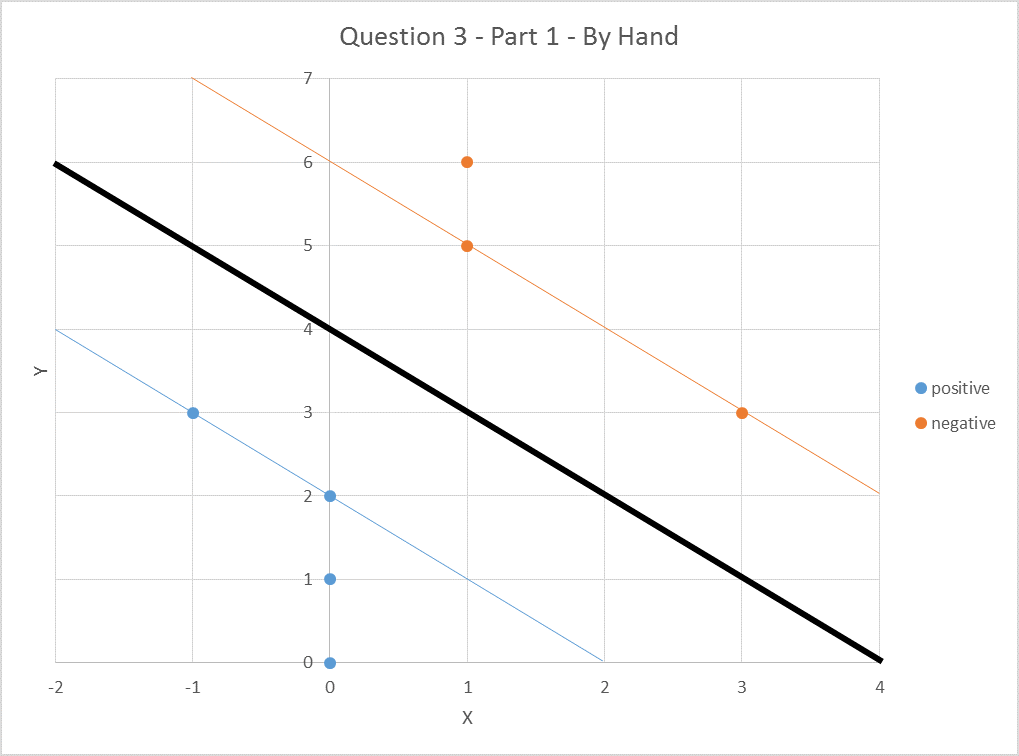
\includegraphics[width=1\textwidth]{question_3_plot_1}
    \caption{Positive data set is blue. Negative data set is orange. Hand drawn linear classifier in black. Support vectors for corresponding data sets also included}
    \label{fig:question_3_plot_1}
\end{figure}

\subsection*{Part b}
The parameters w and b for this line are -1 and 4, respectively. The equation below represents the drawn classifer.
\begin{equation}
h(x) = -x+4
\end{equation}

\subsection*{Part c}
\begin{figure}[H]
    \centering
    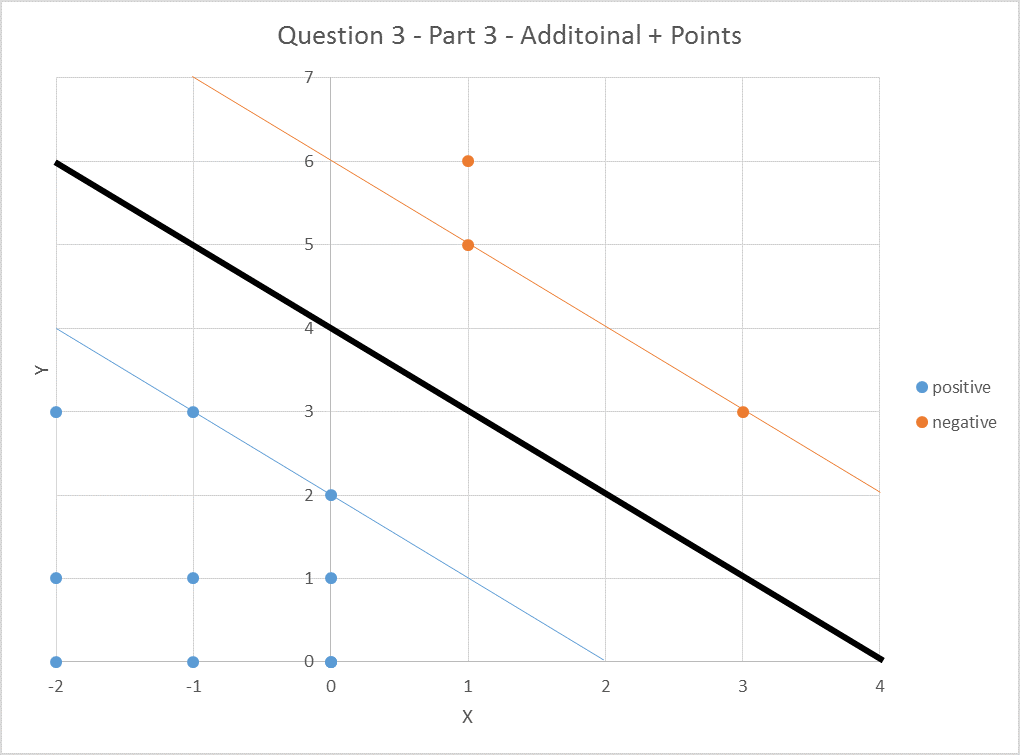
\includegraphics[width=1\textwidth]{question_3_plot_2}
    \caption{Positive data set is blue. Negative data set is orange. Hand drawn linear classifier in black. Support vectors for corresponding data sets also included}
    \label{fig:question_3_plot_2}
\end{figure}
The addition of more data to the positive data set did not change the linear SVM because the values did not change the position of the corresponding support vectors. As a result, the values of w and b are unchanged and the equation below still represents the classifer in the graph.
\begin{equation}
h(x) = -x+4
\end{equation}

\section*{Question 4}

\subsection*{Part a}

\begin{figure}[H]
    \centering
    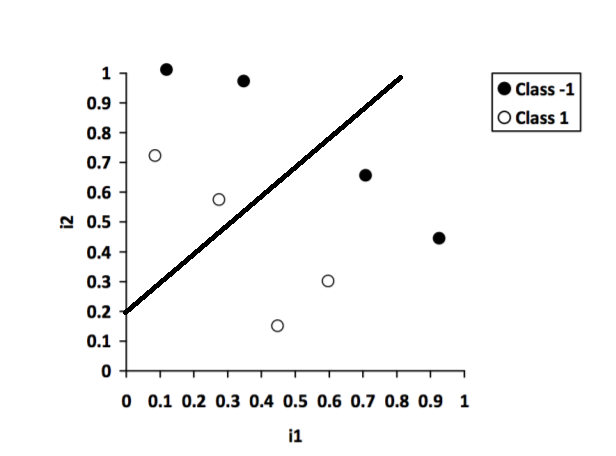
\includegraphics[width=1\textwidth]{question_4_plot_a}
    \caption{The plot with }
    \label{fig:question_4_plot_a}
\end{figure}

\section*{Question 5}

\subsection*{Part a}

\begin{figure}[H]
    \centering
    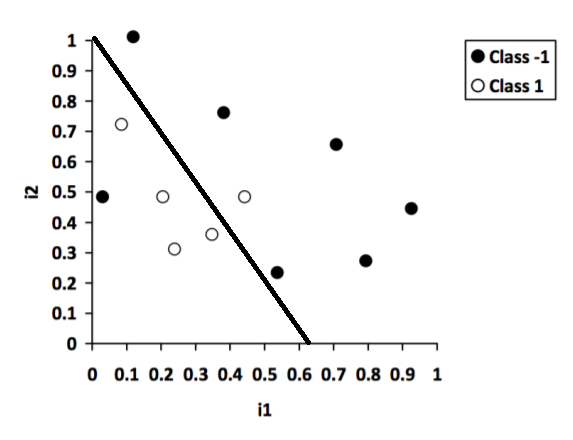
\includegraphics[width=1\textwidth]{question_5_plot_a}
    \caption{The minimum error possible is 2.}
    \label{fig:question_5_plot_a}
\end{figure}

\subsection*{Part b}

\begin{figure}[H]
    \centering
    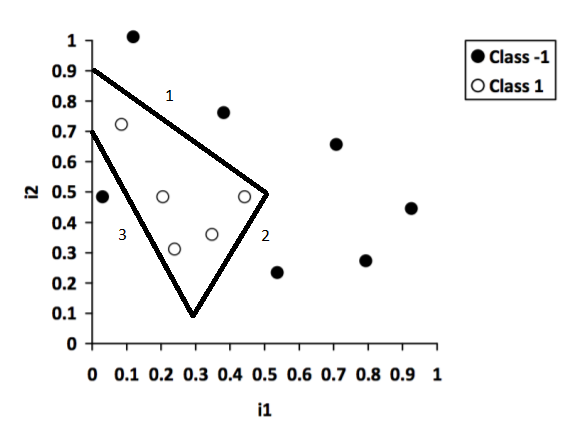
\includegraphics[width=1\textwidth]{question_5_plot_b}
    \caption{A multilayer perceptron with 3 layers separates the two categories.}
    \label{fig:question_5_plot_b}
\end{figure}

The weights for the lines are:
\\
$w_0 = -0.9, w_1 = \frac{4}{7}, w_2 = -1$ for line 1 
\\
$w_0 = -0.08, w_1 = -0.6, w_2 = 1$ for line 2
\\
$w_0 = -0.7, w_1 = 2.5, w_2 = 1$ for line 3

\end{document}